% !TEX root = ../Dokumentation.tex
\subsection{Entladen}
%
\textbf{Funktionsbeschrieb}\\[0.2cm]
\begin{figure}[H]
\centering
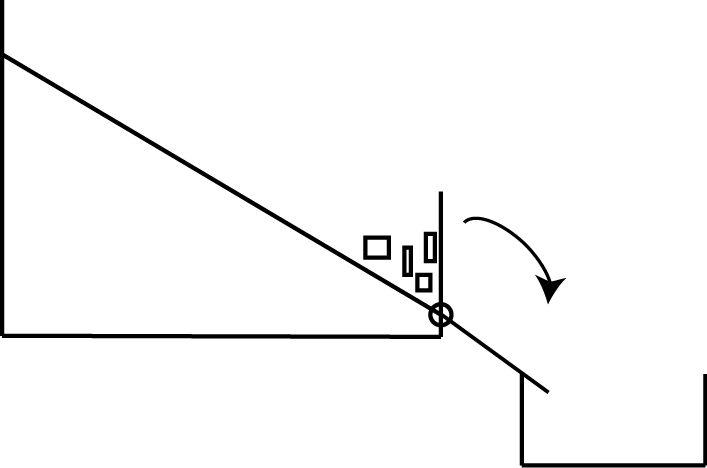
\includegraphics[width=0.5\textwidth]{03_Loesungskonzept/pictures/Entladen_Schraegbehaelter.png}
\caption{Entladen}
\end{figure}\flushleft
%
Beim Entladevorgang fährt das Fahrzeug bis auf 25mm +/- 5mm an den Rand der rechten Seitenlinie. Anschliessend wird die Klappe gelöst und sie fällt auf den Rand des Entsorgungsbeckens. Über die Klappe rutscht das Schüttgut in das Entsorgungsbecken. Nach erfolgter Abladung wird die Klappe wieder nach oben gezogen und ist wieder in der Ausgangsstellung.
%
Damit die Klappe wieder in Ausgangsstellung gebracht werden kann, werden oben rechts bzw. links Bohrungen angebracht. Dort können Seile befestigt werden. Diese werden auf Rollen auf- bzw. abgewickelt. Die beiden Rollen werden auf einer Welle befestigt, die von einem DC-Motor angetrieben wird.\\[0.2cm]
\begin{figure}[H]
\centering
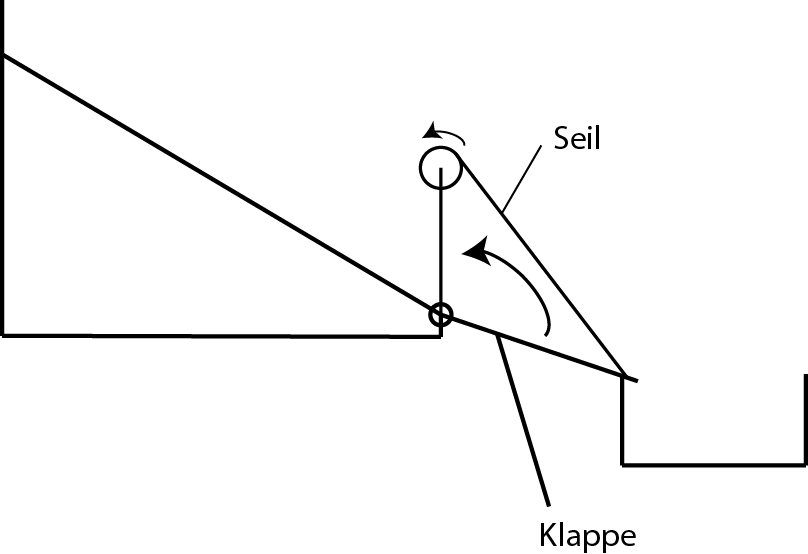
\includegraphics[width=0.5\textwidth]{03_Loesungskonzept/pictures/Klappe_schliessen.png}
\caption{Klappe schliessen}
\end{figure}\flushleft
%
\textbf{Komponentenbeschrieb}\\[0.2cm]
Die Klappe besteht aus einem handelsüblichen Scharnier auf dem eine Platte aus Acrylglas befestigt ist.\\[0.2cm]
%
\textbf{Berechnungen}\\[0.2cm]
DC-Motor für Entladeklappe:
\begin{itemize}
\item $m = 0.15kg$
\item $l = 0.1m$
\item $M = m\cdot g\cdot l = 0.015Nm = 1.5Ncm$
\item Sicherheitsfaktor =2
\item $M = 1.5\cdot 2 = 3Ncm$
\end{itemize} 